\documentclass[11pt,a4paper,oneside]{book}
\usepackage{umcu}
\title{SPARQLing genomics}
\author{Roel Janssen}

\begin{document}

\begin{titlepage}
  \topskip0pt
  \vspace*{\fill}
  \begin{center}
    
\includegraphics[width=0.75\textwidth]{figures/logo.pdf}
    %\Huge SPARQLing genomics
    \rule{0.75\textwidth}{1.0pt}~\\
    %\Large Roel Janssen~\\~\\
    \url{https://github.com/UMCUGenetics/sparqling-genomics}~\\
    \large v0.99.0, \today{}
    % Put it a little bit above the center of the page.
    ~\\~\\~\\~\\~\\~\\~\\~\\~\\~\\~\\~\\~\\~\\
  \end{center}
  \topskip0pt
  \vspace*{\fill}

  \thispagestyle{empty}
\end{titlepage}

\setcounter{page}{1}
\pagenumbering{roman}
\hypersetup{linkcolor=black}
\tableofcontents
\newpage{}
\hypersetup{linkcolor=LinkGray}
\setcounter{page}{1}
\pagenumbering{arabic}

\chapter{Getting started}

  SPARQLing genomics is a combination of tools and practices to create a
  knowledge graph to make \emph{discovering}, \emph{connecting}, and
  \emph{collaborating} easy.

\section{Prerequisites}
\label{sec:prerequisites}

  The programs provided by this project are designed to build a knowledge graph.
  However, a knowledge graph store (better known as an RDF store) is not included
  because various great RDF stores already exist, including
  \href{https://virtuoso.openlinksw.com/}{Virtuoso},
  \href{https://github.com/4store/4store}{4store} and
  \href{https://www.blazegraph.com/}{BlazeGraph}.  We recommend using one of
  the mentioned RDF stores with the programs from this project.

  Before we can use the programs provided by this project, we need to build
  them.  The build system needs
  \href{https://www.gnu.org/software/autoconf}{GNU Autoconf},
  \href{https://www.gnu.org/software/automake}{GNU Automake},
  \href{https://www.gnu.org/software/make}{GNU Make} and
  \href{https://www.freedesktop.org/wiki/Software/pkg-config/}{pkg-config}.
  Additionally, for building the documentation, a working \LaTeX{} distribution is
  required including the \texttt{pdflatex} program.  Because \LaTeX{} distributions
  are rather large, this is dependency is optional, at the cost of not being able
  to (re)generate the documentation.

  Each component in the repository has its own dependencies.  Table
  \ref{table:dependencies} provides an overview for each tool.  A \B{}
  indicates that the program (row) depends on the program or library (column).
  Care was taken to pick dependencies that are widely available on GNU/Linux
  systems.

  \hypersetup{urlcolor=black}
  \begin{table}[H]
    \begin{tabularx}{\textwidth}{X *{9}{!{\color{white}\VRule[1pt]}l}}
      \headrow \cellcolor{White}
      & \rotatebox[origin=l]{90}{\href{https://gcc.gnu.org/}{C compiler}\space\space\space}
      & \rotatebox[origin=l]{90}{\href{http://www.librdf.org/}{raptor2}}
      & \rotatebox[origin=l]{90}{\href{http://www.xmlsoft.org/}{libxml2}}
      & \rotatebox[origin=l]{90}{\href{http://www.htslib.org/}{HTSLib}}
      & \rotatebox[origin=l]{90}{\href{https://zlib.net/}{zlib}}
      & \rotatebox[origin=l]{90}{\href{https://www.gnu.org/software/guile}{GNU Guile}}
      & \rotatebox[origin=l]{90}{\href{https://www.gnutls.org/}{GnuTLS}}
      & \rotatebox[origin=l]{90}{\href{https://tug.org/texlive/}{\LaTeX{}}}\\
      \evenrow
      \texttt{vcf2rdf}         & \B & \B &    & \B &    &    & \B &\\
      \oddrow
      \texttt{bam2rdf}         & \B & \B &    & \B &    &    & \B &\\
      \evenrow
      \texttt{table2rdf}       & \B & \B &    &    & \B &    & \B &\\
      \oddrow
      \texttt{json2rdf}        & \B & \B &    &    & \B &    & \B &\\
      \evenrow
      \texttt{xml2rdf}         & \B & \B & \B &    & \B &    & \B &\\
      \oddrow
      \texttt{folder2rdf}      &    &    &    &    &    & \B &    &\\
      \evenrow
      \texttt{sg-web}          &    &    &    &    &    & \B & \B &\\
      \oddrow
      \texttt{sg-web-test}     &    &    &    &    &    & \B & \B &\\
      \evenrow
      \texttt{sg-auth-manager} &    &    &    &    &    & \B & \B &\\
      \oddrow
      Documentation            &    &    &    &    &    &    &    & \B \\
    \end{tabularx}
    \caption{\small External tools required to build and run the programs of
      this project.}
    \label{table:dependencies}
  \end{table}
  \hypersetup{urlcolor=LinkGray}

  The manual provides example commands to import RDF using
  \href{https://curl.haxx.se/}{cURL}.

\section{Installing the prerequisites}

\subsection{Debian}

  Debian includes all tools, so use this command to install the
  build dependencies:

\begin{siderules}
\begin{verbatim}
apt-get install autoconf automake gcc make pkg-config zlib1g-dev  \
                guile-2.2 guile-2.2-dev libraptor2-dev libhts-dev \
                texlive curl libxml2-dev gnutls-dev
\end{verbatim}
\end{siderules}

  This command has been tested on Debian 10.  If you're using a different
  version of Debian, some package names may differ.

\subsection{CentOS}

  CentOS 7 and 8 do not include \texttt{htslib}.  Follow the instructions on
  the \href{https://www.htslib.org/}{\texttt{htslib} website}%
  \footnote{https://www.htslib.org/} to build \texttt{htslib} from source.

  All other dependencies can be installed using the following command:

\begin{siderules}
\begin{verbatim}
yum install autoconf automake gcc make pkgconfig guile guile-devel \
            raptor2-devel texlive curl libxml2-devel gnutls-devel
\end{verbatim}
\end{siderules}

\subsection{GNU Guix}

  For GNU Guix, use the \texttt{environment.scm} file to set up the development
  environment:

\begin{siderules}
\begin{verbatim}
guix environment -l environment.scm
\end{verbatim}
\end{siderules}

\subsection{MacOS}

  The necessary dependencies to build \texttt{sparqling-genomics} can be
  installed using \href{https://brew.sh/}{homebrew}:

\begin{siderules}
\begin{verbatim}
brew install autoconf automake gcc make pkg-config guile \
             htslib curl raptor libxml2 zlib gnutls
\end{verbatim}
\end{siderules}

  Due to a missing \LaTeX{} distribution on MacOS, the documentation
  cannot be build.

\section{Obtaining the source code}
\label{sec:obtaining-tarball}

  \begin{sloppypar}
  The source code can be downloaded at the
  \href{https://github.com/UMCUGenetics/sparqling-genomics/releases}%
  {Releases}%
  \footnote{\url{https://github.com/UMCUGenetics/sparqling-genomics/releases}}
  page.  Make sure to download the {\fontfamily{\ttdefault}\selectfont
    sparqling-genomics-\sgversion{}.tar.gz} file.
  \end{sloppypar}

  Or, directly download the tarball using the command-line:
\begin{siderules}
\begin{lstlisting}[language=bash]
curl -LO https://github.com/UMCUGenetics/sparqling-genomics/releases/\
download/(@*\sgversion{}*@)/sparqling-genomics-(@*\sgversion{}*@).tar.gz
\end{lstlisting}
\end{siderules}

  After obtaining the tarball, it can be unpacked using the \texttt{tar}
  command:

\begin{siderules}
\begin{lstlisting}
tar zxvf sparqling-genomics-(@*\sgversion{}*@).tar.gz
\end{lstlisting}
\end{siderules}

\section{Installation instructions}

  After installing the required tools (see section \refer{sec:prerequisites}),
  and obtaining the source code (see section \refer{sec:obtaining-tarball}),
  building involves running the following commands:

\begin{siderules}
\begin{lstlisting}
cd sparqling-genomics-(@*\sgversion{}*@)
autoreconf -vif # Only needed if the "./configure" step does not work.
./configure
make
make install
\end{lstlisting}
\end{siderules}

  To run the \texttt{make install} command, super user privileges may be
  required.  This step can be ignored, but will keep the tools in the project's
  directory.  So in that case, invoking \texttt{vcf2rdf} must be done using
  \texttt{tools/vcf2rdf/vcf2rdf} when inside the project's root directory,
  instead of ``just'' \texttt{vcf2rdf}.

  Alternatively, specify a \texttt{-{}-prefix} to the \texttt{configure}
  script to install the tools to a user-writeable location.

  Individual components can be built by replacing \texttt{make} with the
  more specific \texttt{make -C <component-directory>}.  So, to \emph{only}
  build \texttt{vcf2rdf}, the following command could be used:

\begin{siderules}
\begin{verbatim}
make -C tools/vcf2rdf
\end{verbatim}
\end{siderules}

\section{Using a pre-built Docker image}

  A pre-built Docker container can be obtained from the release page.  It
  can be imported into docker using the following commands:

\begin{siderules}
\begin{lstlisting}
curl -LO https://github.com/UMCUGenetics/sparqling-genomics/releases/\
download/(@*\sgversion{}*@)/sparqling-genomics-(@*\sgversion{}*@)-docker.tar.gz
docker load < sparqling-genomics-(@*\sgversion{}*@)-docker.tar.gz
\end{lstlisting}
\end{siderules}

  The container includes both SPARQLing genomics and Virtuoso (open source
  edition).


\chapter{Command-line programs}

  The project provides programs to create a complete pipeline including
  data conversion, data importing and data exploration.  The tasks we can
  perform with the command-line programs are:
  \begin{itemize}
    \item Extract triples from VCF files;
    \item Push data to a SPARQL endpoint.
  \end{itemize}

\section{Preparing variant call data with \texttt{vcf2rdf}}
\label{sec:vcf2rdf}

  Obtaining variants from sequenced data is a task of so called
  \emph{variant callers}.  These programs often output the variants they found
  in the \emph{Variant Call Format} (VCF).  Before we can use the data described
  in this format, we need to extract \emph{knowledge} (in the form of triples)
  from it.

  The \texttt{vcf2rdf} program does exactly this, by converting a VCF file
  into an RDF format.  In section \ref{sec:curl} {\color{LinkGray}`\nameref{sec:curl}%
  '} we describe how to import the data produced by \texttt{vcf2rdf} in the
  database.

\subsection{Knowledge extracted by \texttt{vcf2rdf}}

  The program treats the VCF as its own ontology.  It uses the VCF header as
  a guide.  All fields described in the header of the VCF file will be
  translated into triples.

  In addition to the knowledge from the VCF file, \texttt{vcf2rdf} stores the
  following metadata:

    \begin{table}[H]
    \begin{tabularx}{\textwidth}{ l l l L }
      \headrow
      \textbf{Subject} & \textbf{Predicate} & \textbf{Object}
      & \textbf{Description}\\
      \evenrow
      :Origin & rdf:type & owl:Class
      & \texttt{:Origin} is used to identify a data origin (which
      is usually a file).\\
      \oddrow
      :Sample & rdf:type & owl:Class
      & \texttt{:Sample} is used to identify a sample name.\\
      \evenrow
      :filename & rdf:type & xsd:string
      & \texttt{:filename} contains the path to the file that \texttt{:Origin}
      represents.\\
      \oddrow
      :convertedBy & rdf:type & owl:AnnotationProperty
      & \texttt{:convertedBy} is used to identify the program that performed
      the VCF->RDF conversion.\\
      \evenrow
      :foundIn & rdf:type & owl:AnnotationProperty
      & \texttt{:foundIn} relates the \texttt{:Origin} to a \texttt{:Sample}.\\
    \end{tabularx}
    \caption{\small The additional triple patterns described by \texttt{vcf2rdf}.}
    \label{table:vcf2rdf-ontology}
  \end{table}

  The following snippet is an example of the extra data in Turtle-format:

  \begin{siderules}
\begin{verbatim}
<http://rdf.umcutrecht.nl/vcf2rdf/14f2b609b>
    :convertedBy :vcf2rdf ;
    :filename "clone_ref_tumor.vcf.gz"^^xsd:string ;
    a :Origin .

sample:CLONE_REF
    :foundIn <http://rdf.umcutrecht.nl/vcf2rdf/14f2b609b3> ;
    a :Sample .

sample:CLONE_TUMOR
    :foundIn <http://rdf.umcutrecht.nl/vcf2rdf/14f2b609b3> ;
    a :Sample .
\end{verbatim}
\end{siderules}

\subsection{Example usage}

\begin{siderules}
\begin{verbatim}
vcf2rdf -i /path/to/my/variants.vcf > /path/to/my/variants.ttl
\end{verbatim}
\end{siderules}

\subsection{Run-time properties}

  Depending on the serialization format, the program typically uses from two megabytes
  (in \texttt{ntriples} mode), to multiple times the size of the input VCF
  (in \texttt{turtle} mode).

  The \texttt{ntriples} mode can output triples as soon as they are formed, while the
  \texttt{turtle} mode waits until all triples are known, so that it can output them
  efficiently, producing compact output at the cost of using more memory.

  We recommend using the \texttt{ntriples} format for large input files, and
  \texttt{turtle} for small input files.

\section{Preparing sequence data with \texttt{fasta2rdf}}
\label{sec:fasta2rdf}

  Resources like pre-composed reference genomes are often distributed in the
  FASTA file format.  The \texttt{fasta2rdf} program generates RDF that
  describes each nucleotide, its position (where the first nucleotide is at
  position 1, not 0), and to which sequence the nucleotide belongs.

  Its main aim is to describe a sequence to allow for querying the sequence
  context of a variant.

\subsection{Knowledge extracted by \texttt{fasta2rdf}}

  The \texttt{fasta2rdf} program extracts a nucleotide and describes it along
  with its position in the sequence.

  In addition to the knowledge from the FASTA file, \texttt{fasta2rdf} stores the
  following metadata:

  \begin{table}[H]
    \begin{tabularx}{\textwidth}{ l l l L }
      \headrow
      \textbf{Subject} & \textbf{Predicate} & \textbf{Object}
      & \textbf{Description}\\
      \evenrow
      :Origin & rdf:type & owl:Class
      & \texttt{:Origin} is used to identify a data origin (which
      is usually a file).\\
      \oddrow
      :Sample & rdf:type & owl:Class
      & \texttt{:Sample} is used to identify a sample name.\\
      \evenrow
      :Sequence & rdf:type & owl:Class
      & \texttt{:Sequence} is used to identify a sequence within the file.
      This is typically a chromosome or contig\\
      \oddrow
      :filename & rdf:type & xsd:string
      & \texttt{:filename} contains the path to the file that \texttt{:Origin}
      represents.\\
      \evenrow
      :convertedBy & rdf:type & owl:AnnotationProperty
      & \texttt{:convertedBy} is used to identify the program that performed
      the VCF->RDF conversion.\\
      \oddrow
      :foundIn & rdf:type & owl:AnnotationProperty
      & \texttt{:foundIn} relates the \texttt{:Origin} to a \texttt{:Sample}.\\
    \end{tabularx}
    \caption{\small The additional triple patterns described by \texttt{fasta2rdf}.}
    \label{table:fasta2rdf-ontology}
  \end{table}

  The following snippet is an example of the extra data in Turtle-format:

  \begin{siderules}
\begin{verbatim}
<http://rdf.umcutrecht.nl/fasta2rdf/14f2b609b>
    :convertedBy :vcf2rdf ;
    :filename "grch37.fasta.gz"^^xsd:string ;
    a :Origin .

sample:grch37
    :foundIn <http://rdf.umcutrecht.nl/fasta2rdf/14f2b609b3> ;
    a :Sample .

sample:CLONE_TUMOR
    :foundIn <http://rdf.umcutrecht.nl/fasta2rdf/14f2b609b3> ;
    a :Sample .
\end{verbatim}
\end{siderules}

\section{Importing data with \texttt{curl}}
\label{sec:curl}

  To load RDF data into a triple store (our database), we can use \texttt{curl}.

  The triple stores typically store data in \emph{graphs}.  One triple store
  can host multiple graphs, so we must tell the triple store which graph we
  would like to add the data to.

\subsection{Example usage}

% Other types: application/n-triples
\begin{siderules}
\begin{verbatim}
curl -X POST                                                 \
     -H Content-Type:text/turtle                             \
     -T /path/to/variants.ttl                                \
     -G <endpoint URL>                                       \
     --digest -u <username>:<password>                       \
     --data-urlencode graph=http://example/graph
\end{verbatim}
\end{siderules}

\chapter{Web interface}
\label{chap:web-interface}

  In addition to the command-line programs, the project provides a web
  interface for prototyping queries, and quick data reporting.  With the
  web interface you can:
  \begin{itemize}
  \item Write and execute SPARQL queries;
  \item Keep track of different SPARQL endpoints.
  \end{itemize}

\section{Running the web interface}

  The web interface can be started using the \texttt{sg-web} command:

\begin{siderules}
\begin{verbatim}
sg-web
\end{verbatim}
\end{siderules}

  By default, it will be accessible on \url{http://localhost:5000}.

\subsection{Configurating connections}

  The first useful step is to configure a connection to a SPARQL endpoint.

  \begin{figure}[h]
    \begin{center}
      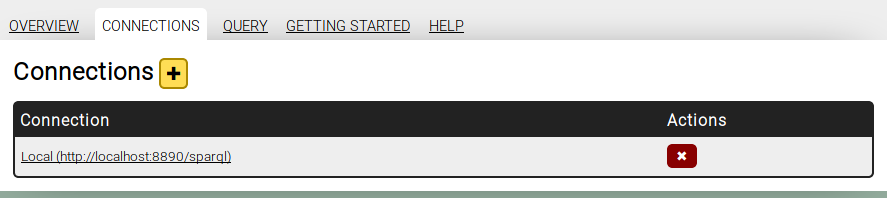
\includegraphics[width=1.0\textwidth]{figures/web-connections.png}
    \end{center}
    \caption{The \emph{connections} page enables users to configure accessible
      SPARQL endpoints.  Adding a connection here will provide an option to
      query it on the \emph{query} page.}
    \label{fig:web-connections}
  \end{figure}

  When providing a username and password for a connection, it will attempt
  to connect using \emph{digest authentication}.

\subsection{Executing queries}

  After configuring at least one endpoint, it can be chosen on the \emph{query}
  page to execute a query against it.

  \begin{figure}[h]
    \begin{center}
      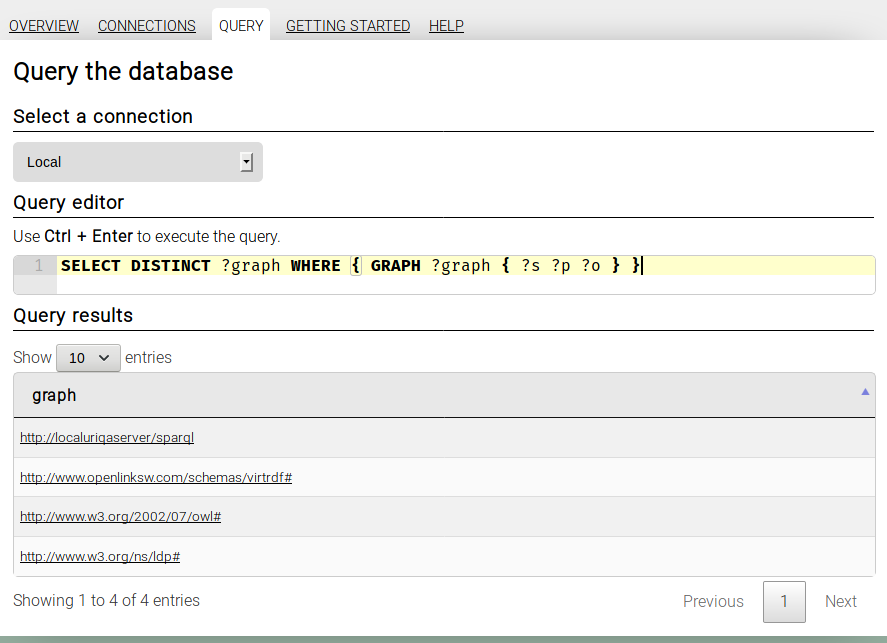
\includegraphics[width=1.0\textwidth]{figures/web-query.png}
    \end{center}
    \caption{The \emph{query} page enables users to execute a query against a
      SPARQL endpoint.  The connections configured at the \emph{connections} page
      can be chosen from the drop-down menu.}
    \label{fig:web-query}
  \end{figure}

\chapter{Information retrieval with SPARQL}

  In section \ref{sec:vcf2rdf} {\color{LinkGray}`%
  \nameref{sec:vcf2rdf}'} we discussed how to extract triples from common data
  formats.  In section \ref{sec:curl} {\color{LinkGray}`\nameref{sec:curl}'} we
  discussed how we could insert those triples into a SPARQL endpoint.

  In this section, we will start exploring the inserted data by using a
  query language called \emph{SPARQL}.  Understanding SPARQL will be crucial
  for the integration in your own programs or scripts --- something we will
  discuss in chapter \ref{chap:programming} {\color{LinkGray}%
  `\nameref{chap:programming}'}.

  The queries in the remainder of this chapter can be readily copy/pasted into
  the query editor of the web interface (see chapter \ref{chap:web-interface}
  {\color{LinkGray}`\nameref{chap:web-interface}'}).

\section{Local querying}

  The promise from ``linked data'' is to make data available in such a way that
  one query can retrieve information from multiple SPARQL endpoints.  We call
  querying over multiple SPARQL endpoints \emph{federated querying}.  But before
  we do that, let's look at simple queries that only look at our own data.

\subsection{Listing non-empty graphs}
\label{sec:non-empty-graphs}
  Each SPARQL endpoint can host multiple \emph{graphs}.  Each graph can contain
  an independent set of triples.  The following query displays the available
  graphs in a SPARQL endpoint:

\begin{siderules}
\begin{verbatim}
SELECT DISTINCT ?graph WHERE { GRAPH ?graph { ?s ?p ?o } }
\end{verbatim}
\end{siderules}

\subsection{Querying a specific graph}

  The sooner we can reduce the dataset to query over, the faster the query will
  return with an answer.  One easy way to reduce the size of the dataset is to
  be specific about which graph to query.  This can be achieved using the
  \texttt{FROM} clause in the query.

\begin{siderules}
\begin{verbatim}
SELECT ?s ?p ?o
FROM <graph-name>
WHERE { ?s ?p ?o }
\end{verbatim}
\end{siderules}

  Without the \texttt{FROM} clause, the RDF store will search in all graphs.
  We can repeat the \texttt{FROM} clause to query over multiple graphs in the
  same RDF store.

\begin{siderules}
\begin{verbatim}
SELECT ?s ?p ?o
FROM <graph-name>
FROM <another-graph-name>
WHERE { ?s ?p ?o }
\end{verbatim}
\end{siderules}

  In section \ref{sec:federated-querying} {\color{LinkGray}%
  `\nameref{sec:federated-querying}'} we will look at querying over multiple
  RDF stores.

\subsection{Exploring the structure of knowledge in a graph}

  Inside the \texttt{WHERE} clause of a SPARQL query we specify a graph
  pattern.  One useful method of finding out which patterns exist in a
  graph is to look for predicates:

\begin{siderules}
\begin{verbatim}
SELECT DISTINCT ?predicate
FROM <graph-name>
WHERE {
  ?subject ?predicate ?object .
}
\end{verbatim}
\end{siderules}

  The \texttt{graph-name} must be one of the graphs returned by the query from
  section \ref{sec:non-empty-graphs} {\color{LinkGray}%
    `\nameref{sec:non-empty-graphs}'}.

\subsection{Listing samples and their originating files}

Using the knowledge we gained from exploring the predicates in a graph,
we can construct more insightful queries, like finding the names of the
samples and their originating filenames from the output of \texttt{vcf2rdf}:

\begin{siderules}
\begin{verbatim}
PREFIX vcf2rdf: <http://rdf.umcutrecht.nl/vcf2rdf/>

SELECT DISTINCT STRAFTER(STR(?sample), "Sample/") AS ?sample ?filename
FROM <graph-name>
WHERE {
  ?variant  vcf2rdf:sample    ?sample .
  ?sample   vcf2rdf:foundIn   ?origin .
  ?origin   vcf2rdf:filename  ?filename .
}
\end{verbatim}
\end{siderules}

\subsection{Listing samples, originated files, and number of variants}

Building on the previous query, and by exploring the predicates of a
\texttt{vcf2rdf:VariantCall}, we can construct the following query to
include the number of variants for each sample, in each file.

\begin{siderules}
\begin{verbatim}
PREFIX vcf2rdf: <http://rdf.umcutrecht.nl/vcf2rdf/>
PREFIX rdf: <http://www.w3.org/1999/02/22-rdf-syntax-ns#>

SELECT DISTINCT STRAFTER(STR(?sample), "Sample/") AS ?sample
       ?filename
       COUNT(DISTINCT ?variant) AS ?numberOfVariants

FROM <graph-name>
WHERE
{
  ?variant  rdf:type                vcf2rdf:VariantCall ;
            vcf2rdf:sample          ?sample ;
            vcf2rdf:originatedFrom  ?origin .

  ?origin   vcf2rdf:filename        ?filename .
}
\end{verbatim}
\end{siderules}

  By using \texttt{COUNT}, we can get the \texttt{DISTINCT} number of
  matching patterns for a variant call for a sample, originating from
  a distinct file.

\subsection{Retrieving all variants}

  When retrieving potentially large amounts of data, the \texttt{LIMIT}
  clause may come in handy to prototype a query until we are sure enough
  that the query answers the actual question we would like to answer.

  In the next example query, we will retrieve the sample name,
  chromosome, position, and the corresponding VCF \texttt{FILTER} field(s)
  from the database.

\begin{siderules}
\begin{verbatim}
PREFIX vcf2rdf: <http://rdf.umcutrecht.nl/vcf2rdf/>
PREFIX vc: <http://rdf.umcutrecht.nl/vcf2rdf/VariantCall/>
PREFIX rdf: <http://www.w3.org/1999/02/22-rdf-syntax-ns#>
PREFIX faldo: <http://biohackathon.org/resource/faldo#>

SELECT DISTINCT ?variant ?sample ?chromosome ?position ?filter
FROM <graph-name>
WHERE
{
  ?variant  rdf:type                vcf2rdf:VariantCall ;
            vcf2rdf:sample          ?sample ;
            faldo:reference         ?chromosome ;
            faldo:position          ?position ;
            vc:FILTER               ?filter .
}
LIMIT 100
\end{verbatim}
\end{siderules}

  By limiting the result set to the first 100 rows, the query will return
  with an answer rather quickly.  Had we not set a limit to the number of
  rows, the query could have returned possibly a few million rows, which
  would obviously take longer to process.

\section{Federated querying}
\label{sec:federated-querying}

  Now that we've seen local queries, there's only one more construct we need to
  know to combine this with remote SPARQL endpoints: the \texttt{SERVICE}
  construct.

  For the next example, we will use the \href{http://www.ebi.ac.uk/rdf/services/sparql}%
  {public SPARQL endpoint hosted by EBI}.

\subsection{Get an overview of Biomodels (from ENSEMBL)}
\begin{siderules}
\begin{verbatim}
PREFIX sbmlrdf: <http://identifiers.org/biomodels.vocabulary#>
PREFIX sbmldb: <http://identifiers.org/biomodels.db/>

SELECT ?speciesId ?name {
  SERVICE <http://www.ebi.ac.uk/rdf/services/sparql/> {
    sbmldb:BIOMD0000000001 sbmlrdf:species ?speciesId .
    ?speciesId sbmlrdf:name ?name
  }
}
\end{verbatim}
\end{siderules}

\chapter{Programming in Python, Perl, R, Scheme, C, and/or C++}
\label{chap:programming}

\section{Using SPARQL with R}
\label{sec:sparql-with-r}

  Before we can start, we need to install the \texttt{SPARQL} package from
  \href{https://cran.r-project.org/web/packages/SPARQL/index.html}{CRAN}.

\begin{siderules}
\begin{verbatim}
install.packages('SPARQL')
\end{verbatim}
\end{siderules}

  Once we're set up, we can query like so:

\begin{siderules}
\begin{verbatim}
# Load the library
library('SPARQL')

# Define the endpoint to query.
endpoint <- "http://localhost:8890/sparql"

# Define the actual query to run.
query <- "PREFIX vcf2rdf: <http://rdf.umcutrecht.nl/vcf2rdf/>
PREFIX vc: <http://rdf.umcutrecht.nl/vcf2rdf/VariantCall/>
PREFIX rdf: <http://www.w3.org/1999/02/22-rdf-syntax-ns#>
PREFIX faldo: <http://biohackathon.org/resource/faldo#>

SELECT DISTINCT ?variant ?sample ?chromosome ?position ?filter
FROM <graph-name>
WHERE
{
  ?variant  rdf:type                vcf2rdf:VariantCall ;
            vcf2rdf:sample          ?sample ;
            faldo:reference         ?chromosome ;
            faldo:position          ?position ;
            vc:FILTER               ?filter .
}
LIMIT 10";

# Run the query
query_data <- SPARQL (endpoint, query)

# Put the results (a data frame) in a separate variable.
query_results <- query_data$results
\end{verbatim}
\end{siderules}

\end{document}
